% 0277(본책 53쪽) — 원 O, 현 AB=14 cm(수선의 발 M, OM=x cm), 현 CD=14 cm(수선의 발 N), OM=ON 같은 변 표시, OD=9 cm. 답(x)은 적지 않는다. 스캔 삽화를 TikZ 로 다시 그림.
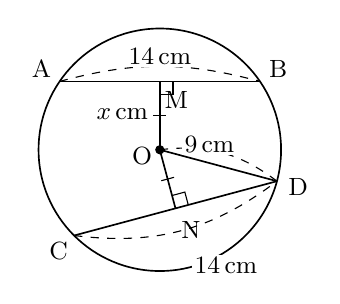
\begin{tikzpicture}[scale=1.4, line width=0.6pt]
  \draw (0.000,0.000) circle (1.100);
  \draw (-0.909,0.620) -- (0.909,0.620);
  \draw (-0.778,-0.778) -- (1.063,-0.285);
  \draw (0.000,0.000) -- (0.000,0.620);
  \draw (0.000,0.000) -- (0.142,-0.531);
  \draw (0.000,0.000) -- (1.063,-0.285);
  \fill (0.000,0.000) circle (1.2pt);
  \draw[line width=0.4pt] (0.120,0.620) -- (0.120,0.500) -- (0.000,0.500);
  \draw[line width=0.4pt] (0.258,-0.500) -- (0.227,-0.384) -- (0.111,-0.415);
  \draw[line width=0.4pt] (-0.060,0.310) -- (0.060,0.310);
  \draw[line width=0.4pt] (0.129,-0.250) -- (0.013,-0.281);
  \draw[dashed, line width=0.4pt] (-0.909,0.620) to[bend left=15] (0.909,0.620);
  \node[font=\small, fill=white, inner sep=1pt] at (0.000,0.850) {$14\,\mathrm{cm}$};
  \node[font=\small, fill=white, inner sep=1pt] at (-0.340,0.320) {$x\,\mathrm{cm}$};
  \draw[dashed, line width=0.4pt] (0.000,0.000) to[bend left=22] (1.063,-0.285);
  \node[font=\small, fill=white, inner sep=1pt] at (0.450,0.050) {$9\,\mathrm{cm}$};
  \draw[dashed, line width=0.4pt] (-0.778,-0.778) to[bend right=22] (1.063,-0.285);
  \node[font=\small, fill=white, inner sep=1pt] at (0.600,-1.050) {$14\,\mathrm{cm}$};
  \node[font=\small, inner sep=1.5pt] at (-0.160,-0.060) {O};
  \node[font=\small, inner sep=1.5pt] at (-1.074,0.733) {A};
  \node[font=\small, inner sep=1.5pt] at (1.074,0.733) {B};
  \node[font=\small, inner sep=1.5pt] at (-0.919,-0.919) {C};
  \node[font=\small, inner sep=1.5pt] at (1.256,-0.336) {D};
  \node[font=\small, inner sep=1.5pt] at (0.150,0.450) {M};
  \node[font=\small, inner sep=1.5pt] at (0.282,-0.731) {N};
\end{tikzpicture}
